\subsection{Proceso de Mapeo del Modelo Entidad--Relación al Modelo Relacional}
\label{subsec:mapeo_er_mr}

\subsubsection{1. Breve descripción del proyecto}
El proyecto consiste en el desarrollo de una plataforma web diseñada para organizar, centralizar y dar seguimiento continuo al proceso de tesis en programas de posgrado universitario\cite{sim2023technology}. La herramienta busca resolver de manera directa tres problemáticas frecuentes en el acompañamiento tutorial:
\begin{itemize}
    \item \textbf{Control de versiones de borradores:} Permite la recepción de entregables únicamente en formato PDF para garantizar la estabilidad del contenido, resguardando cada archivo con un correlativo de versión inmutable (sin sobreescritura ni eliminación accidental de revisiones pasadas)\cite{iso32000, chacon2014progit}.
    \item \textbf{Formalización de minutas de asesoría:} Ofrece un registro digital estructurado para asentar la fecha, modalidad y temas tratados en cada sesión de trabajo, junto con la lista de acuerdos y tareas pendientes asignadas tanto al estudiante como al asesor\cite{pmi2021}.
    \item \textbf{Monitoreo y prevención del rezago escolar:} Implementa un mecanismo automatizado que calcula los días transcurridos desde el último avance o minuta registrada, emitiendo alertas visuales preventivas cuando el tesista rebasa los 30 días de inactividad académica\cite{lando2025digital}.
\end{itemize}

\subsubsection{2. Diagrama Entidad--Relación de partida}
El proceso de transformación toma como entrada directa el modelo conceptual desarrollado en la subsección~\ref{subsec:diagrama_eer} (Figura~\ref{fig:diagrama_relacional}). En dicho esquema se identificaron entidades fuertes regulares (\texttt{usuario}, \texttt{proyecto\_tesis}, \texttt{minutas\_asesoria}, \texttt{alerta\_rezago}), entidades débiles dependientes de existencia e identificación (\texttt{entregable\_version}, \texttt{compromiso\_acuerdo}), jerarquías de especialización por rol (\texttt{alumno}, \texttt{asesor}, \texttt{coordinador}), atributos compuestos, atributos multivaluados (\texttt{telefono}) y un atributo derivado (\texttt{dias\_inactividad}).

\subsubsection{3. Proceso detallado de transformación por reglas de mapeo}
Para convertir el esquema conceptual en un conjunto coherente de tablas relacionales se aplicaron formalmente las reglas de mapeo descritas por Silberschatz et al.\cite{silberschatz2014}:

\paragraph{Paso 1: Mapeo de entidades fuertes regulares}
\textbf{Regla utilizada:} Por cada entidad fuerte regular del diagrama se crea una relación (tabla). Los atributos simples pasan a ser columnas directas y el atributo identificador clave se define como llave primaria (\textit{Primary Key}, PK). 

Si la entidad cuenta con atributos compuestos, estos se dividen en sus componentes elementales más pequeños. Los atributos derivados no se reservan como columnas fijas en la tabla, ya que su valor se obtiene dinámicamente mediante consultas temporales en el sistema.

\begin{enumerate}
    \item \textbf{Entidad \texttt{usuario}:} Se establece \texttt{id\_usuario} como su llave primaria. El atributo compuesto \texttt{nombre\_completo} se descompone en \texttt{primer\_nombre}, \texttt{segundo\_nombre}, \texttt{apellido\_paterno} y \texttt{apellido\_materno}. El atributo multivaluado \texttt{telefono} se extrae para procesarse en un paso posterior.
    \begin{quote}
        \textbf{Tabla creada:} \\
        \texttt{USUARIO}(\underline{id\_usuario}, primer\_nombre, segundo\_nombre, apellido\_paterno, apellido\_materno, correo\_institucional, contrasena, fecha\_registro, cuenta\_activa)
    \end{quote}

    \item \textbf{Entidad \texttt{proyecto\_tesis}:} Se define \texttt{id\_proyecto} como llave primaria. El atributo derivado \texttt{dias\_inactividad} se omite como campo físico en la tabla base, pues se calcula en tiempo real restando la fecha del último avance de la fecha actual del sistema.
    \begin{quote}
        \textbf{Tabla creada:} \\
        \texttt{PROYECTO\_TESIS}(\underline{id\_proyecto}, titulo\_tesis, linea\_investigacion, fecha\_inicio, fecha\_ultimo\_avance, estado\_proyecto)
    \end{quote}

    \item \textbf{Entidad \texttt{minutas\_asesoria}:} Se asigna \texttt{id\_minuta} como llave primaria.
    \begin{quote}
        \textbf{Tabla creada:} \\
        \texttt{MINUTAS\_ASESORIA}(\underline{id\_minuta}, fecha\_reunion, modalidad, resumen\_temas, fecha\_registro)
    \end{quote}

    \item \textbf{Entidad \texttt{alerta\_rezago}:} Se toma \texttt{id\_alerta} como llave primaria.
    \begin{quote}
        \textbf{Tabla creada:} \\
        \texttt{ALERTA\_REZAGO}(\underline{id\_alerta}, fecha\_deteccion, dias\_acumulados, estado\_alerta)
    \end{quote}
\end{enumerate}

\paragraph{Paso 2: Mapeo de especialización y generalización (Jerarquía de usuarios)}
\textbf{Regla utilizada:} Para una especialización con superclase general y subclases disjuntas, se implementa una tabla separada para cada subclase. La llave primaria de cada subtipo se conforma por la misma llave primaria de la superclase (\texttt{id\_usuario}), fungiendo a la vez como llave foránea (\textit{Foreign Key}, FK) hacia la tabla padre. Cada tabla hija almacena únicamente los atributos exclusivos de su rol funcional.

\begin{enumerate}
    \item \textbf{Subclase \texttt{alumno}:}
    \begin{quote}
        \textbf{Tabla creada:} \\
        \texttt{ALUMNO}(\underline{id\_usuario}, matricula) \\
        \textit{Llave foránea (FK):} \texttt{id\_usuario} $\rightarrow$ \texttt{USUARIO(id\_usuario)}
    \end{quote}

    \item \textbf{Subclase \texttt{asesor}:}
    \begin{quote}
        \textbf{Tabla creada:} \\
        \texttt{ASESOR}(\underline{id\_usuario}, numero\_empleado, grado\_academico) \\
        \textit{Llave foránea (FK):} \texttt{id\_usuario} $\rightarrow$ \texttt{USUARIO(id\_usuario)}
    \end{quote}

    \item \textbf{Subclase \texttt{coordinador}:}
    \begin{quote}
        \textbf{Tabla creada:} \\
        \texttt{COORDINADOR}(\underline{id\_usuario}, cubiculo\_oficina, telefono\_oficina) \\
        \textit{Llave foránea (FK):} \texttt{id\_usuario} $\rightarrow$ \texttt{USUARIO(id\_usuario)}
    \end{quote}
\end{enumerate}

\paragraph{Paso 3: Mapeo de atributos multivaluados}
\textbf{Regla utilizada:} Por cada atributo multivaluado presente en el diagrama, se crea una tabla nueva e independiente. La llave primaria de esta tabla se construye de forma compuesta, integrando la llave foránea que apunta a la entidad propietaria junto con el valor propio del atributo multivaluado.

\begin{itemize}
    \item \textbf{Atributo \texttt{telefono} de la entidad \texttt{usuario}:} Permite registrar uno o más números telefónicos por usuario sin generar duplicidad de filas en la tabla principal.
    \begin{quote}
        \textbf{Tabla creada:} \\
        \texttt{USUARIO\_TELEFONO}(\underline{id\_usuario}, \underline{numero\_telefono}) \\
        \textit{Llave foránea (FK):} \texttt{id\_usuario} $\rightarrow$ \texttt{USUARIO(id\_usuario)}
    \end{quote}
\end{itemize}

\paragraph{Paso 4: Mapeo de relaciones binarias $1:1$ y $1:N$}
\textbf{Reglas utilizadas:}
\begin{itemize}
    \item \textbf{Relaciones $1:1$:} La llave primaria de la entidad participante con rol independiente se añade como llave foránea en la tabla subordinada, agregando una restricción de unicidad (\textit{UNIQUE}) para garantizar que no se asocie a más de un registro.
    \item \textbf{Relaciones $1:N$:} La llave primaria de la entidad ubicada en el lado ``$1$'' de la relación se incorpora como llave foránea dentro de la tabla del lado ``$N$''.
\end{itemize}

\begin{enumerate}
    \item \textbf{Relación $1:1$ Desarrolla (\texttt{alumno} $\leftrightarrow$ \texttt{proyecto\_tesis}):} Cada alumno desarrolla un único proyecto y cada proyecto le corresponde a un solo alumno. Se inserta \texttt{id\_alumno} como llave foránea con restricción única en \texttt{PROYECTO\_TESIS}.
    \item \textbf{Relación $1:N$ Dirige (\texttt{asesor} $\leftrightarrow$ \texttt{proyecto\_tesis}):} Un asesor dirige múltiples proyectos de tesis. Se agrega \texttt{id\_asesor} como llave foránea en \texttt{PROYECTO\_TESIS}.
    \item \textbf{Relación $1:N$ Supervisa (\texttt{coordinador} $\leftrightarrow$ \texttt{proyecto\_tesis}):} El coordinador supervisa todos los proyectos registrados. Se agrega \texttt{id\_coordinador} como llave foránea en \texttt{PROYECTO\_TESIS}.
    \begin{quote}
        \textbf{Tabla modificada (\texttt{PROYECTO\_TESIS}):} \\
        \texttt{PROYECTO\_TESIS}(\underline{id\_proyecto}, titulo\_tesis, linea\_investigacion, fecha\_inicio, fecha\_ultimo\_avance, estado\_proyecto, id\_alumno, id\_asesor, id\_coordinador) \\
        \textit{FK 1:} \texttt{id\_alumno} $\rightarrow$ \texttt{ALUMNO(id\_usuario)} [Única] \\
        \textit{FK 2:} \texttt{id\_asesor} $\rightarrow$ \texttt{ASESOR(id\_usuario)} \\
        \textit{FK 3:} \texttt{id\_coordinador} $\rightarrow$ \texttt{COORDINADOR(id\_usuario)}
    \end{quote}

    \item \textbf{Relación $1:N$ Registra (\texttt{proyecto\_tesis} $\leftrightarrow$ \texttt{minutas\_asesoria}):} Un proyecto de tesis agrupa un historial de múltiples sesiones de asesoría. Se agrega \texttt{id\_proyecto} en la tabla de minutas.
    \begin{quote}
        \textbf{Tabla modificada (\texttt{MINUTAS\_ASESORIA}):} \\
        \texttt{MINUTAS\_ASESORIA}(\underline{id\_minuta}, fecha\_reunion, modalidad, resumen\_temas, fecha\_registro, id\_proyecto) \\
        \textit{Llave foránea (FK):} \texttt{id\_proyecto} $\rightarrow$ \texttt{PROYECTO\_TESIS(id\_proyecto)}
    \end{quote}

    \item \textbf{Relación $1:N$ Dispara aviso (\texttt{proyecto\_tesis} $\leftrightarrow$ \texttt{alerta\_rezago}):} Un proyecto acumula avisos periódicos por inactividad académica prolongada. Se agrega \texttt{id\_proyecto} en la tabla de alertas.
    \begin{quote}
        \textbf{Tabla modificada (\texttt{ALERTA\_REZAGO}):} \\
        \texttt{ALERTA\_REZAGO}(\underline{id\_alerta}, fecha\_deteccion, dias\_acumulados, estado\_alerta, id\_proyecto) \\
        \textit{Llave foránea (FK):} \texttt{id\_proyecto} $\rightarrow$ \texttt{PROYECTO\_TESIS(id\_proyecto)}
    \end{quote}
\end{enumerate}

\paragraph{Paso 5: Mapeo de entidades débiles}
\textbf{Regla utilizada:} Por cada tipo de entidad débil se crea una relación (tabla). Su llave primaria estará conformada por la llave primaria de la entidad fuerte de la cual depende (que actúa como llave foránea) unida al discriminante o clave parcial de la entidad débil.

\begin{enumerate}
    \item \textbf{Entidad débil \texttt{entregable\_version}:} Depende existencialmente de la entidad fuerte \texttt{proyecto\_tesis}. Su discriminante local es el campo \texttt{numero\_version}.
    \begin{quote}
        \textbf{Tabla creada:} \\
        \texttt{ENTREGABLE\_VERSION}(\underline{id\_proyecto}, \underline{numero\_version}, ruta\_archivo\_pdf, fecha\_hora\_subida, comentario\_alumno, retroalimentacion\_asesor) \\
        \textit{Llave foránea (FK):} \texttt{id\_proyecto} $\rightarrow$ \texttt{PROYECTO\_TESIS(id\_proyecto)}
    \end{quote}

    \item \textbf{Entidad débil \texttt{compromiso\_acuerdo}:} Depende de la entidad \texttt{minutas\_asesoria}. Su discriminante es el correlativo \texttt{numero\_acuerdo}.
    \begin{quote}
        \textbf{Tabla creada:} \\
        \texttt{COMPROMISO\_ACUERDO}(\underline{id\_minuta}, \underline{numero\_acuerdo}, descripcion\_tarea, responsable, fecha\_limite, estado\_cumplido) \\
        \textit{Llave foránea (FK):} \texttt{id\_minuta} $\rightarrow$ \texttt{MINUTAS\_ASESORIA(id\_minuta)}
    \end{quote}
\end{enumerate}


\subsection{Esquema y Diagrama Relacional Resultante}
\label{subsec:esquema_diagrama_relacional}

Una vez concluidas todas las etapas de transformación conceptual, el sistema queda estructurado en 10 tablas relacionales. Este diseño elimina redundancias de datos, preserva la integridad referencial y permite una implementación directa sobre un motor relacional como MySQL o PostgreSQL.

\subsubsection{Listado formal de tablas y atributos}
A continuación, se detalla el catálogo completo de relaciones, indicando con subrayado (\underline{PK}) las llaves primarias simples o compuestas, y especificando las llaves foráneas (\textit{FK}) asociadas:

\begin{enumerate}
    \item \textbf{USUARIO}(\underline{id\_usuario}, primer\_nombre, segundo\_nombre, apellido\_paterno, apellido\_materno, correo\_institucional, contrasena, fecha\_registro, cuenta\_activa)
    
    \item \textbf{USUARIO\_TELEFONO}(\underline{id\_usuario}, \underline{numero\_telefono}) \\
    \textit{FK:} \texttt{id\_usuario} $\rightarrow$ \texttt{USUARIO(id\_usuario)}.
    
    \item \textbf{ALUMNO}(\underline{id\_usuario}, matricula) \\
    \textit{FK:} \texttt{id\_usuario} $\rightarrow$ \texttt{USUARIO(id\_usuario)}.
    
    \item \textbf{ASESOR}(\underline{id\_usuario}, numero\_empleado, grado\_academico) \\
    \textit{FK:} \texttt{id\_usuario} $\rightarrow$ \texttt{USUARIO(id\_usuario)}.
    
    \item \textbf{COORDINADOR}(\underline{id\_usuario}, cubiculo\_oficina, telefono\_oficina) \\
    \textit{FK:} \texttt{id\_usuario} $\rightarrow$ \texttt{USUARIO(id\_usuario)}.
    
    \item \textbf{PROYECTO\_TESIS}(\underline{id\_proyecto}, titulo\_tesis, linea\_investigacion, fecha\_inicio, fecha\_ultimo\_avance, estado\_proyecto, id\_alumno, id\_asesor, id\_coordinador) \\
    \textit{FK 1:} \texttt{id\_alumno} $\rightarrow$ \texttt{ALUMNO(id\_usuario)} (\textit{Restricción Unique}). \\
    \textit{FK 2:} \texttt{id\_asesor} $\rightarrow$ \texttt{ASESOR(id\_usuario)}. \\
    \textit{FK 3:} \texttt{id\_coordinador} $\rightarrow$ \texttt{COORDINADOR(id\_usuario)}.
    
    \item \textbf{ENTREGABLE\_VERSION}(\underline{id\_proyecto}, \underline{numero\_version}, ruta\_archivo\_pdf, fecha\_hora\_subida, comentario\_alumno, retroalimentacion\_asesor) \\
    \textit{FK:} \texttt{id\_proyecto} $\rightarrow$ \texttt{PROYECTO\_TESIS(id\_proyecto)}.
    
    \item \textbf{MINUTAS\_ASESORIA}(\underline{id\_minuta}, fecha\_reunion, modalidad, resumen\_temas, fecha\_registro, id\_proyecto) \\
    \textit{FK:} \texttt{id\_proyecto} $\rightarrow$ \texttt{PROYECTO\_TESIS(id\_proyecto)}.
    
    \item \textbf{COMPROMISO\_ACUERDO}(\underline{id\_minuta}, \underline{numero\_acuerdo}, descripcion\_tarea, responsable, fecha\_limite, estado\_cumplido) \\
    \textit{FK:} \texttt{id\_minuta} $\rightarrow$ \texttt{MINUTAS\_ASESORIA(id\_minuta)}.
    
    \item \textbf{ALERTA\_REZAGO}(\underline{id\_alerta}, fecha\_deteccion, dias\_acumulados, estado\_alerta, id\_proyecto) \\
    \textit{FK:} \texttt{id\_proyecto} $\rightarrow$ \texttt{PROYECTO\_TESIS(id\_proyecto)}.
\end{enumerate}

\subsubsection{Diagrama Relacional}
En la Figura~\ref{fig:diagrama_relacional} se presenta el modelo físico-relacional del sistema, donde se aprecian las tablas con sus tipos de datos, sus llaves primarias señaladas con llave dorada y las conexiones de llaves foráneas que garantizan la consistencia referencial de toda la información almacenada.

\begin{figure}[htbp]
    \centering
    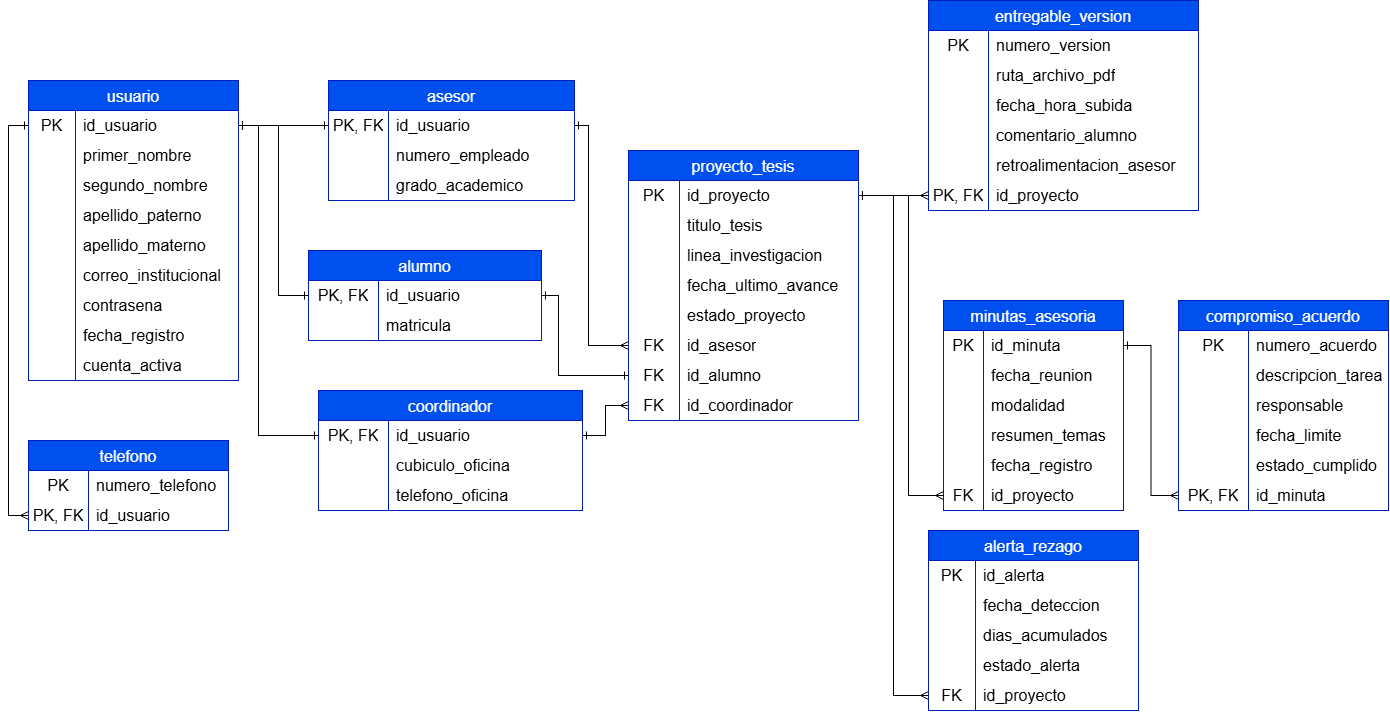
\includegraphics[width=0.95\textwidth]{assets/database/diagrama_relacional.png}
    \caption{Diagrama Relacional de la base de datos para la plataforma de seguimiento de tesis.}
    \label{fig:diagrama_relacional}
\end{figure}